\chapter{Способы решения проблемы возврата регенерированного урана}\label{ch:ch3}

\section{Разработка схем полного возврата}\label{sec:ch2/sec3}
\subsection{Модифицированный двойной каскад}

В качестве модификации двойного каскада была предложена альтернативная каскадная схема, которая позволяет обеспечить возврат регенерата в цикл в требуемом соотношении. В этой схеме, изображенной 
на рисунке \ref{fig:vestnik}, первая часть (каскад 1) увеличивает 
концентрацию $^{235}$U со всеми более легкими изотопами ($^{232}$U и $^{234}$U) и направляет их на вход второго каскада, который, в свою очередь, в легкой фракции будет концентрировать эти четные миноры в потоке загрязненного продукта \cite{smirnovObogashchenieRegenerirovannogoUrana2018}.
Изотопный же состав получаемый на выходе тяжелой фракции второго каскада, разбавляется НОУ-разбавителем, приготовленным из материала, не содержащего четных искусственных изотопов (ранее не облучаемого в реакторе) -- природного или обедненного урана -- для контроля концентраций $^{232}$U и $^{234}$U в допустимых пределах и для управления соотношением рециклируемых материалов (для поддержания соотношения регенерата в питании каскада к нарабатываемому продукту на требуемом уровне, который формально соответствует эквивалентному возврату (1:1) выгоревшего топлива в ядерный топливный цикл).

\begin{figure}[ht]
  \centerfloat{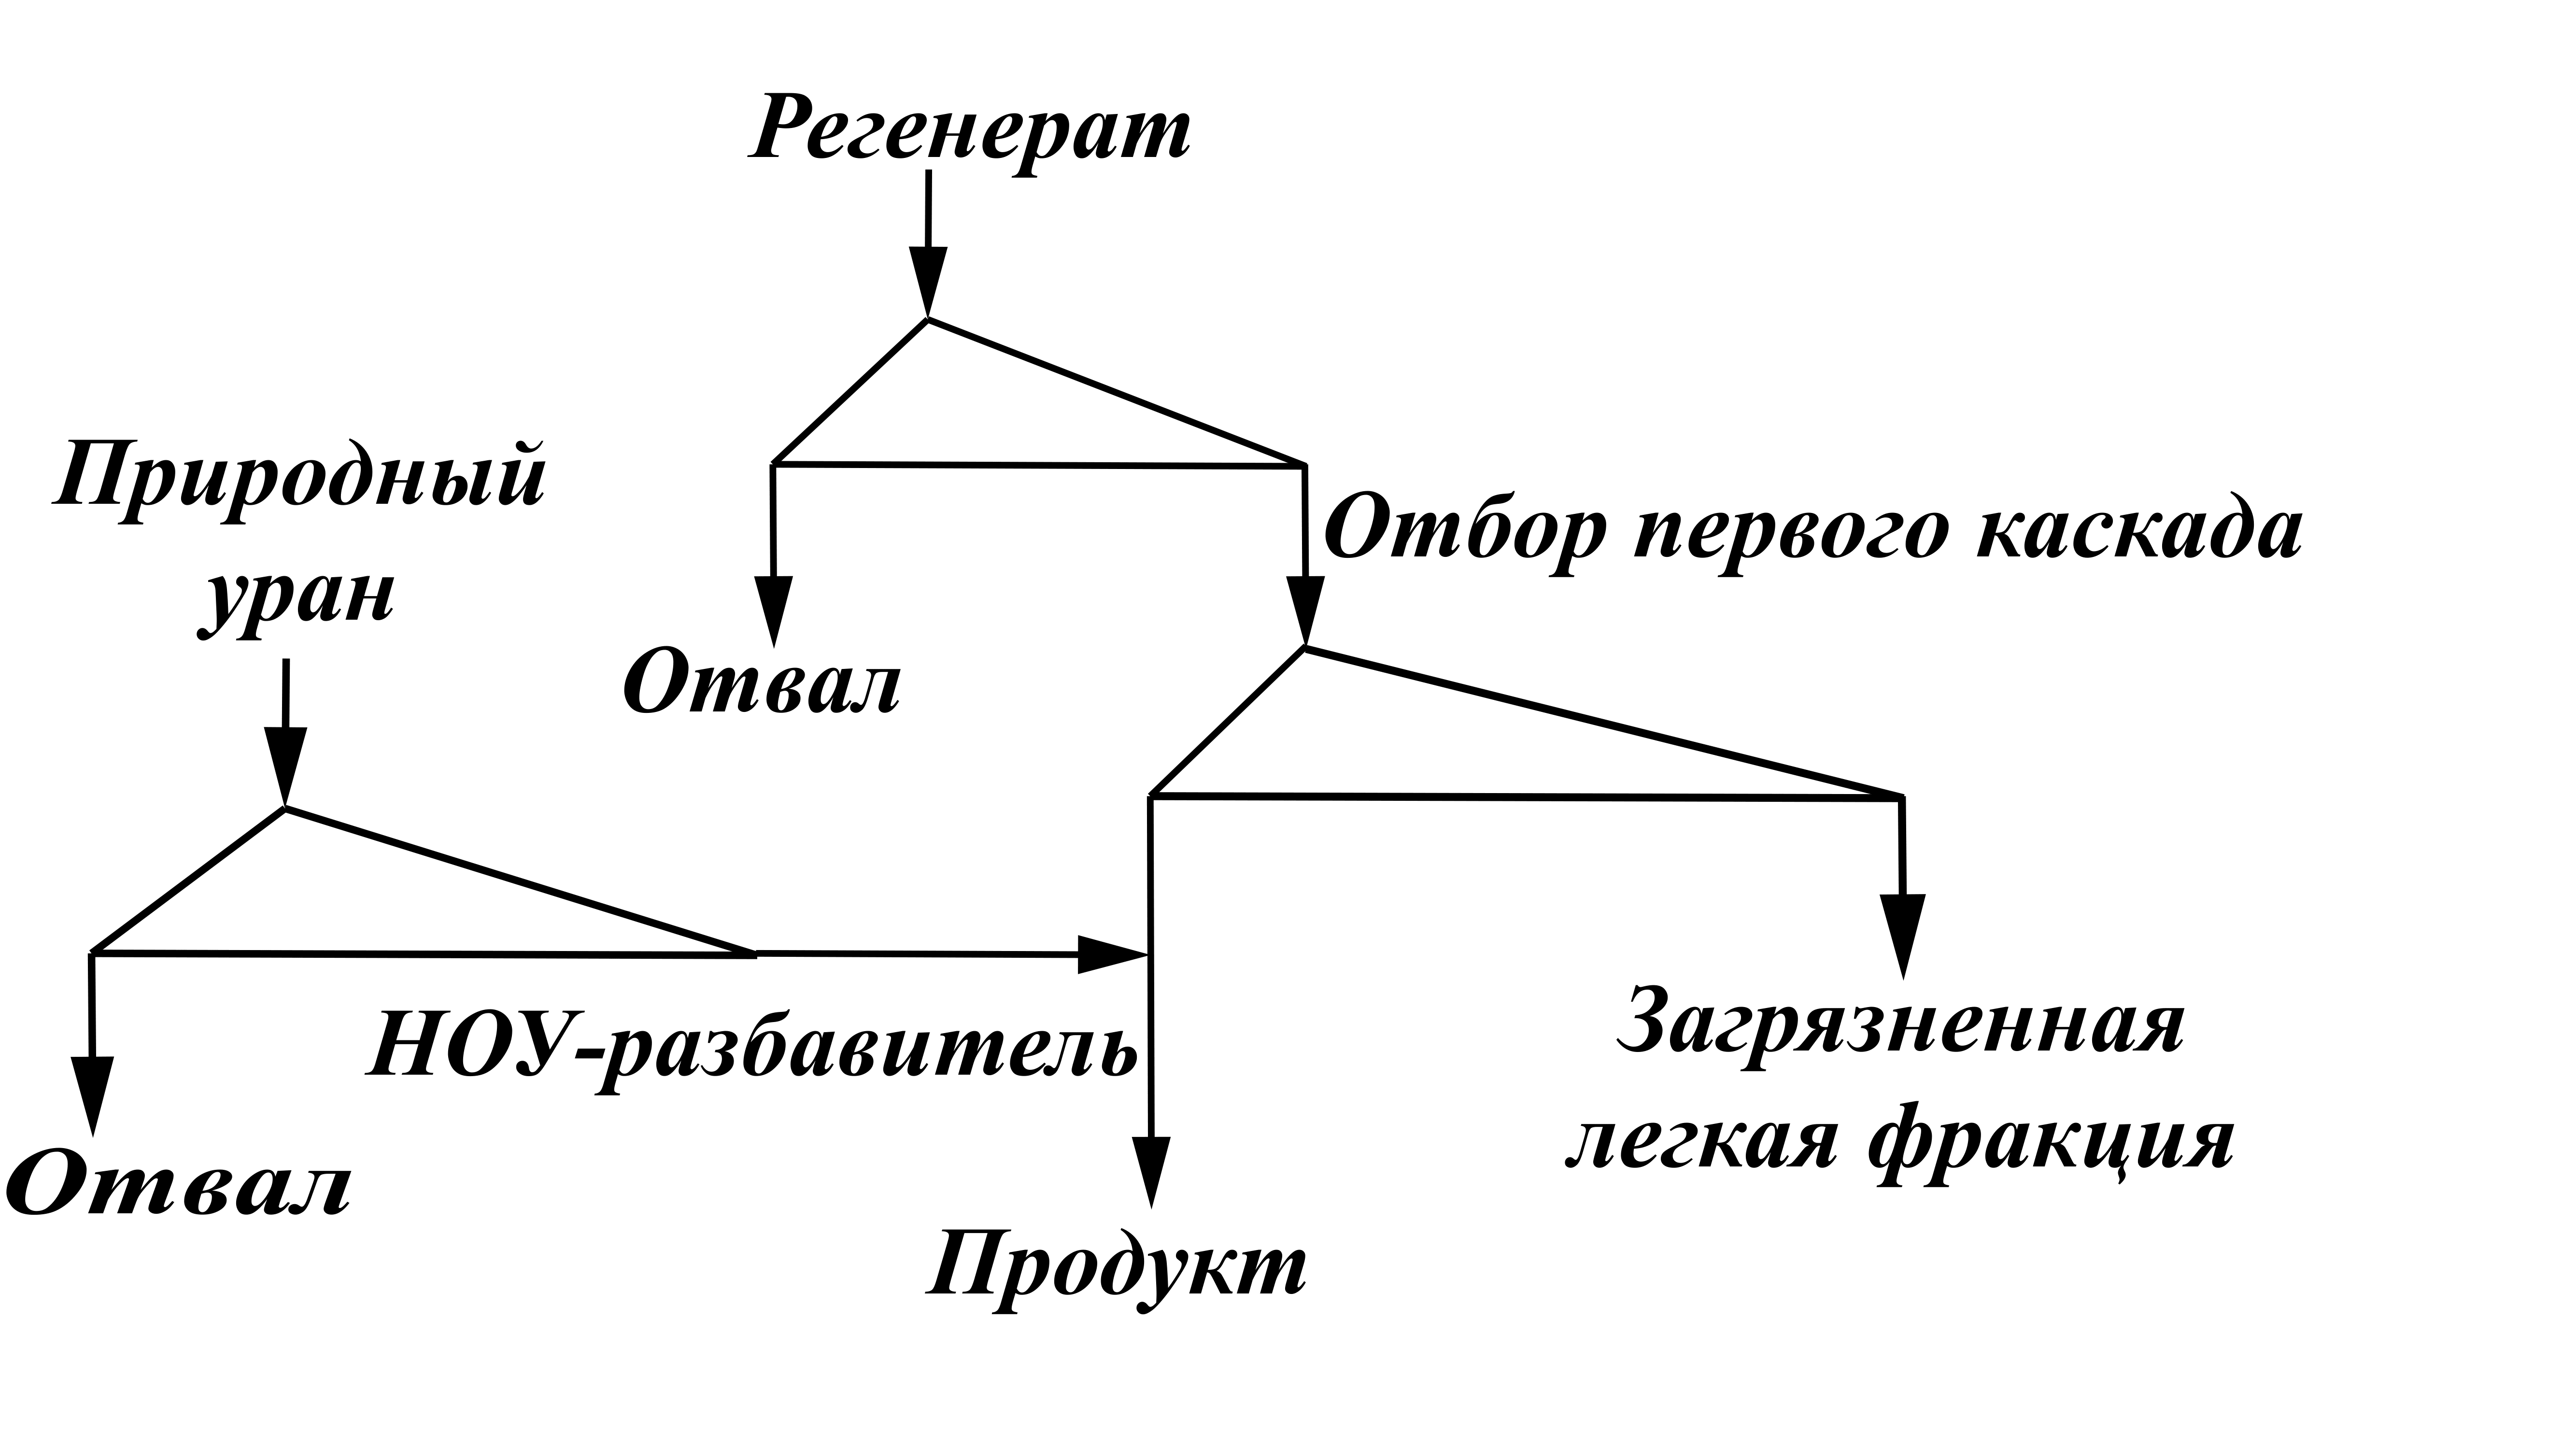
\includegraphics[scale=0.08]{cascades/triple}}
  \caption{Двойной каскад с добавлением НОУ (тройной каскад)}\label{fig:vestnik}
\end{figure}

Отличие предлагаемой схемы от двойного каскада (рис. \ref{fig:double_ru}) состоит в том, что поток отвала второго каскада не является конечным продуктом.
Финальным шагом получения товарного продукта является разбавление этого потока сырьём, не содержащим искусственных изотопов урана с целью их разбавления и, соответственно, обеспечения заданных ограничений по $^{232,236}$U.
Для выполнения условия полного возврата регенерата в цикл, отношение потоков НОУ-разбавителя и отвала второго каскада, которые образуют товарный продукт, является предопределённым, поскольку при заданной концентрации выходящих потоков обоих каскадов известным является отношение потока тяжелой фракции второго каскада к питающему регенерату, и при этом условиями задачи предопределено отношение потока исходного регенерата к конечному-НОУ.
В этом случае единственным параметром, позволяющим влиять на концентрацию $^{235}$U в товарном продукте, является концентрация данного изотопа в разбавителе (в потоке НОУ-разбавитель на рис. \ref{fig:vestnik}).
Таким образом, величину обогащения $^{235}$U в потоке этого разбавителя подбирают для конкретных заданных внешних условий \cite{smirnovObogashchenieRegenerirovannogoUrana2018}.

Очевидно, что, поскольку питанием первого каскада является исходный регенерат, а питанием второго -- полученный из него среднеобогащённый регенерат, то поток тяжёлой фракции на выходе из второго каскада будет по величине в несколько раз меньше, чем исходный поток регенерата. Такая работа каскада обеспечивает перерасход регенерата на единицу продукта. Следовательно, поток разбавителя должен в несколько раз превосходить по величине поток тяжелой фракции второго каскада. Однако, если в качестве разбавителя использовать, например, природный уран, это условие может привести к снижению концентрации $^{235}$U ниже требуемой величины. Если же в качестве разбавителя использовать низкообогащённый уран, то можно увеличить отношение потоков НОУ-разбавителя к <<отвалу>> второго каскада, доведя ее до требуемого значения.  
Такая схема близка к описанной в патенте \cite{zhurinSposobIzotopnogoVosstanovleniya2010}. Однако отличием предлагаемого двойного каскада является то, что ни в одном из каскадов в схеме не происходит превышение концентрации $^{235}$U выше значения 20\%. При этом в схеме  \cite{zhurinSposobIzotopnogoVosstanovleniya2010} концентрация $^{235}$U в потоке P1 достигает 90\% и более. Кроме того, величина отношения потока регенерата к конечному продукту на рис. \ref{fig:vestnik} всегда является строго заданной, что позволяет расходовать на получение заданного количества продукта требуемое количество регенерированного урана.

Итак, согласно \cite{smirnovObogashchenieRegenerirovannogoUrana2018} схема, представленная на рис. \ref{fig:vestnik}, позволяет обогатить регенерированный уран, полученный после пяти рециклов в топливе реакторов ВВЭР-1000 при соотношении расхода регенерата и продукта 0,93 и ограничении на концентрацию $^{232}$U соответствующему значению $5\cdot10^{-7}$\%. Представляет интерес анализ возможности обогащения регенерата в такой схеме при заданном соотношении между массами исходного регенерата и продукта больше единицы. Такое заданное условие моделирует ситуацию обогащения и вовлечения в воспроизводство топлива регенерированного урана, накопленного к текущему моменту за период эксплуатации легководных реакторов. Дополнительный интерес представляет анализ поведения характеристик подобной схемы в зависимости от ограничений на концентрацию изотопа $^{232}$U в продукте. 

\subsubsection{Анализ влияния ограничений предельно допустимой концентрации $^{232}$U в товарном НОУ}

Далее представлены результаты расчёта параметров модификации двойного каскада, представленной на рис. \ref{fig:vestnik}, для различных ограничений на концентрацию изотопа $^{232}$U в продукте, а также соотношения между расходами исходного регенерата и получаемым товарным НОУ.
Согласно цели диссертации, состоящей в исследовании возможностей полного возврата регенерата в режиме многократного рецикла, в качестве сырья для обогащения был рассмотрен регенерированный уран, испытавший несколько циклов облучения (табл. \ref{244549}) \cite{palkinDesignanalyticalResearchRefinement2010}.

Расчёты проведены при следующих условиях: обогащение по изотопу $^{235}$ составляло 4,95\%; относительный коэффициент разделения компонентов $^{235}UF_6$ и $^{238}UF_6$ принят равным 1,2 \cite{smirnovObogashchenieRegenerirovannogoUrana2018}; предельно допустимая концентрация изотопа $^{232}$ в НОУ не должна превышать величины $5\cdot10^{-7}$\%, $2\cdot10^{-7}$\%,$1\cdot10^{-7}$\%; потеря реактивности из-за присутствия $^{236}$U скомпенсирована добавочным обогащением по $^{235}$U; рассматривался состав обогащаемого регенерированного урана пятого рецикла \ref{244549}. Заданный расход регенерированного урана на единицу продукта принят равным:
а) 0,93 кг на 1 кг,
б) 1,86 кг на 1 кг продукта.
Цели расчетов:
\begin{enumerate}
  \item оценка возможности применения рассматриваемой схемы для указанных условий;
  \item оценка влияния изменения внешних условий на интегральные параметры рассматриваемого двойного каскада.
\end{enumerate}

В качестве расчётной модели в настоящей работе использована модель <<квазиидеального>> каскада \cite{sazykinKvaziidealnyeKaskadyDlya2000} с несмешиванием по относительным концентрациям выбранной пары компонентов (R-каскада) \cite{sulaberidzeTeoriyaKaskadovDlya2011}.
Ключевые интегральные характеристики для сравнения: удельный расход природного урана, удельные затраты работы разделения и отношение потока легкой фракции второго каскада к конечному продукту. В приведённых ниже результатах под работой разделения имели в виду условную величину, пропорциональную числу газовых центрифуг в каскаде. 

При этом в каждом каскаде были выбраны следующие пары компонентов, по которым было выполнено условие несмешивания их относительных концентраций: первый каскад $^{235}U$/$^{236}U$, второй каскад $^{235}U$/$^{234}U$.

Концентрацию $^{235}U$ в потоке $P_1$ варьировали в пределах 5--20\% с шагом 1\%, в качестве рабочего значения для каждого случая выбирали величину, обеспечивающую выполнение ограничения на содержание $^{235}U$ в разбавителе, полученном из природного урана, не более 5,0\%. Для такого значения будет наблюдаться минимум по затратам работы разделения, экономии природного урана и отношению потоков $\frac{P_2}{P_0}$. Последнее условие означает, что будет произведено наименьшее количество загрязнённого $^{232}U$, $^{234}U$ изотопами материала $P_2$, хранение которого требует определённых процедур, поскольку он представляет собой повышенную по отношению к штатным отходам разделительных производств опасность.

В табл. \ref{table_PDK_double_modified} представлены результаты расчёта изотопных составов,
в табл. \ref{table3_PDK_double_modified} -- удельный расход природного урана и интегральные характеристики экономии природного урана и перерасхода работы разделения по сравнению с ординарным каскадом, питаемым природным ураном, получающим продукт с эквивалентной эффективной концентрацией $^{235}$U (табл. \ref{table3_PDK_double_modified}). Под работой разделения понимается условная величина, пропорциональная числу газовых центрифуг в каскаде.
 Далее представлены соотношения получаемого загрязненного потока легкой фракции второго каскада к итоговому продукту.

\begin{table}
\begin{tabular}{|c|c|c|c|}
  \hline \multirow{2}{*} {Maccoвoe число} & 
  \multicolumn{3}{|c|}
  {Ограничение по изотопу $^{232} \mathrm{U}$, $\times 10^{-7}$} \\
  \cline {2-4} & 1 & 2 & 5 \\
  \hline \multicolumn{4}{|c|} {Случай $1\left(E_{1} / P_{0}=0,93\right)$} \\
  232 & $1,00 \cdot 10^{-7}$ & $2,00 \cdot 10^{-7}$ & $5,00 \cdot 10^{-7}$ \\
  233 & $2,12 \cdot 10^{-7}$ & $3,62 \cdot 10^{-7}$ & $7,41 \cdot 10^{-7}$ \\
  234 & $4,90 \cdot 10^{-2}$ & $5,30 \cdot 10^{-2}$ & $6,21 \cdot 10^{-2}$ \\
  235 & 5,06 & 5,09 & 5,14 \\
  236 & $3,70 \cdot 10^{-1}$ & $4,67 \cdot 10^{-1}$ & $6,61 \cdot 10^{-1}$ \\
  \hline \multicolumn{4}{|c|} {Случай $2\left(E_{1} / P_{0}=1,86\right)$} \\
  232 & $1,00 \cdot 10^{-7}$ & $2,00 \cdot 10^{-7}$ & $5,00 \cdot 10^{-7}$ \\
  233 & $2,40 \cdot 10^{-7}$ & $4,12 \cdot 10^{-7}$ & $8,55 \cdot 10^{-7}$ \\
  234 & $5,09 \cdot 10^{-2}$ & $5,60 \cdot 10^{-2}$ & $6,79 \cdot 10^{-2}$ \\
  235 & 5,10 & 5,15 & 5,24 \\
  236 & $5,26 \cdot 10^{-1}$ & $6,73 \cdot 10^{-1}$ & $9,85 \cdot 10^{-1}$ \\
  \hline
  \end{tabular}
  \caption{Изотопные составы продукта в модифицированном двойном каскаде для различных условий}\label{table_PDK_double_modified}
\end{table}

\begin{table}
\begin{tabular}{|c|c|c|c|c|}
  \hline
  \makecell{$^{235}$U в \\ потоке  \\ отбора  \\первого  \\каскада, \%} & \makecell{Экономия \\природного  \\ урана, \%} & \makecell{Перерасход \\ работы  \\ разделения, \%} & \makecell{Отношение \\ потока  отбора \\второго каскада \\ к продукту}
  & \makecell{Ограничение  \\ по изотопу $^{232}$U \\ , $\times 10^{-7}$} \\
  \hline
  \multicolumn{5}{|c|} {Случай $1\left(E_{1} / P_{0}=0,93\right)$} \\
  11 & 4,9 & 17,2 & 0,02785 & 1 \\
  10 & 6,7 & 14,7 & 0,02201 & 2 \\
  8 & 10,3 & 9,7 & 0,01038 & 5 \\
  \multicolumn{5}{|c|} {Случай $2\left(E_{1} / P_{0}=1,86\right)$} \\
  13 & 6,6818 & 39,0985 & 0,06648 & 1 \\
  12 & 9,2857 & 35,4797 & 0,05798 & 2 \\
  10 & 14,7795 & 27,7759 & 0,04005 & 5 \\
  \hline
  \end{tabular}
  \caption{Интегральные параметры рассматриваемого двойного каскада для различных внешних условий}\label{table3_PDK_double_modified}
\end{table}


Анализ результатов таблицы \ref{table_PDK_double_modified}  показывает, что рассматриваемая модификация двойного каскада позволяет многократно обогатить регенерированный уран при различных внешних ограничениях, касающихся концентрации $^{232}$U в продукте и величины потока возвращаемого в воспроизводство топлива регенерированного урана.
При этом уменьшение допустимой концентрации $^{232}$U в продукте при фиксированном отношении исходного регенерата к товарному НОУ обусловливает существенное снижение экономии природного урана и изменение числа центрифуг в каскадной схеме.
Например, при отношении регенерата к конечному продукту на уровне 0,93 экономия природного урана уменьшилась, а перерасход работы разделения увеличился примерно в 2 раза при изменении ограничения на $^{232}$U от $5\cdot10^{-7}$\% до $1\cdot10^{-7}$\%. Однако введение более жёстких ограничений на $^{232}$U способствовало одновременному снижению концентрации и остальных чётных изотопов в получаемом продукте, особенно $^{236}$U. Данный фактор является положительным в случае многократного рециклирования урана, поскольку будет обеспечивать меньшее содержание $^{232}$U на последующих рециклах \cite{smirnovObogashchenieRegenerirovannogoUrana2018}.

В рамках настоящей работы рассматривали случай, когда данная концентрация не превышала 20\%, что соответствует порогу, принятому МАГАТЭ для материала прямого использования \cite{alekseevConceptUseRecycled2010}. Однако в некоторых работах, в которых рассматривают двойные каскады для обогащения регенерата, указанная концентрация заметно (в 2 раза и более) превышает величину 20\%. Увеличение данной концентрации, возможно, позволит уменьшить количество получаемого радиоактивного отхода, а также обеспечить более эффективное удаление $^{232}$U из продукта.

Таким образом, использование модифицированного двойного каскада с добавленным потоком НОУ-разбавителя для перемешивания с одним из выходящих потоков второго каскада позволяет успешно обогащать многократно рециклированный уран с максимальным возвратом его в воспроизводство при различных ограничениях на концентрацию изотопа $^{232}$U в продукте, включая более строгие ограничения, чем приняты в настоящее время на заводах по фабрикации топлива для реакторов на тепловых нейтронах.

Хотя этот вариант каскада (рис. \ref{fig:vestnik}) и кажется идеальным, цена хранения побочного продукта из загрязненной смеси может быть неприемлемо высока, что мгновенно сделает схему нежизнеспособной, если нет способов избежать такого негативного побочного эффекта.

\subsection{Тройной каскад}
Итак, в прошлом подразделе, в качестве необходимой модификации двойного каскада была предложена схема каскада рис. \ref{fig:vestnik}, которая позволяет решить проблему возврата необходимого количества регенерата в цикл.

Хотя этот вариант и кажется подходящим для решения поставленной задачи, остается нерешенной судьба легкой фракции второго каскада из-за того, что хранение загрязненного побочного продукта может быть сопряжено с существенными дополнительными затратами, поэтому важен поиск способов избежать накопления этого материала.
Исходя из этого, в диссертационной работе предложено применить дополнительный каскад для утилизации потока загрязненной фракции.

Далее будет предложен краткий обзор такой каскадной схемы.
 
Итак, в \cite{smirnovMethodEnrichReprocessed2019}  было предложено применять дополнительный каскад для производства НОУ из загрязненной смеси, сильно разбавленной обедненным ураном (которые имеют высокую концентрацию $^{235}$U около $\approx$20\%), чтобы получить конечный продукт в двух исходящих потоках и достичь значительной экономии природного урана ($\approx$38\%) даже для <<грязной>> композиции, которая уже была пятикратно рециклирована (рис. \ref{fig:Tomsk}). Расчеты показали, что такой подход позволяет производить НОУ коммерческого качества, расходуя определенное количество переработанного урана и отвечая стандартным спецификациям для  $^{232}$U (и условиям, установленным для других четных изотопов). В то же время, предлагаемая схема обеспечивает большую экономию природного урана, чем большинство схем обогащения переработанного урана. Это могло бы также обеспечить широкомасштабную <<мобилизацию>> обедненного урана.

\begin{figure}[ht]
  \centerfloat{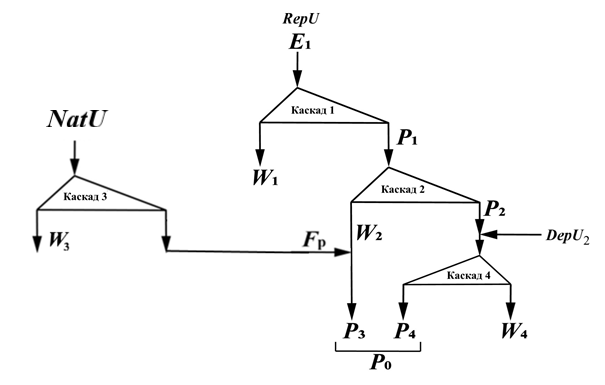
\includegraphics[scale=0.9]{cascades/triple_t}}
  \caption{Тройной каскад с подмешиванием ОГФУ и НОУ-разбавителем}\label{fig:Tomsk}
\end{figure}

Схема такого каскада, состоящего из четырех ординарных каскадов, решает проблему обращения с легкой фракцией, вышедшей из второго каскада.
Это позволяет вовлечь больше $^{235}$U, и избавляет от необходимости конечной утилизации материала с высоким содержанием $^{232}$U.
Принцип работы такой схемы состоит в следующем.
Теперь финальный продукт -- низкообогащенный уран -- получается путем смешения двух потоков.
Первый из них аналогичен финальному продукту, полученному посредством двойного модифицированного каскада.
Второй же нарабатывается из загрязненной смеси, сильно разбавленной обедненным ураном.
При этом, конфигурация подбирается таким образом, чтобы на получение единицы продукта из этих совмещенных потоков затрачивалось требуемое количество ($\approx$0.93) питающего регенерата.

Итак, данная схема позволяет получить конечный НОУ-продукт требуемого качества, смешав два производящих потока и достичь значительной экономии природного урана ($\approx$38\%) даже для «грязного» регенерата, который уже  пятикратно был рециклирован.
При этом, для того же исходного состава регенерата, схема двойного модифицированного каскада (рис. \ref{fig:vestnik}) показывает лишь ($\approx$8\%) в сокращении расхода природного урана в сравнении с ординарным, обогащающим природный уран \cite{smirnovObogashchenieRegenerirovannogoUrana2018}.
Однако, такой эффект связан с двухкратным перерасходом работы разделения в схеме тройного каскада, тогда как в схеме двойного модифицированного каскада затрачивается лишь ($\approx$13\%) дополнительной работы разделения.
Это связано с большим объемом вовлечения ОГФУ для разбавления загрязненного потока легкой фракции второго каскада.
Расчеты показали, что такой подход позволяет производить НОУ коммерческого качества, расходуя должное количество переработанного урана, в то же время отвечая стандартным спецификациям $^{232}$U (и условиям, установленным для других четных изотопов).
В то же время, предлагаемая схема обеспечивает более существенную экономию природного урана, чем большинство схем обогащения регенерированного урана.
Такая схема позволяет также обеспечить широкомасштабную «мобилизацию» обедненного урана.

\section{Сравнение схем полного возврата}

Чтобы проиллюстрировать преимущества и недостатки различных рассмотренных ранее схем, предназначенных для возврата регенерированного урана в ЯТЦ, в данной части диссертационной работы проводится их сравнительный анализ, помогающий сделать предварительные технико-экономические оценки.
Для этого, ключевые характеристики, связанные с общей эффективностью, такие как экономия природного урана, расход работы разделения и энергозатраты, были оценены для каждой схемы в удельных единицах (на единицу продукции).
Затем они были нормированы на величины, характерные для ординарного каскада(трехпоточного).
Чтобы избежать стоимостных показателей затрат, была использована методология пересчета ключевых показателей (экономия природного урана, объем обогащаемого ОГФУ и затраты работы разделения) в единицы потребляемой энергии (мегаватт-часы)  \cite{rodionovaAnalizTehnikoekonomicheskihHarakteristik2019}.
Этот показатель и был предложен в качестве универсального инструмента оценки рассматриваемых каскадов, используемых для повторного обогащения урана.

Концентрация $^{235}$U в потоках отбора второго каскада ограничена уровнем 19,99\% (чтобы не превышать пороговое значение концентрации $^{235}$U для низкообогащенного урана). Для каждого каскада с индексом 2 опорный компонент составляет $^{236}$U и $^{238}$U -- для остальных каскадов.

В качестве схемы №1 рассматривается двойной каскад (рис. \ref{fig:double_ru}), в качестве схемы №2 -- двойной модифицированный (рис. \ref{fig:vestnik}), а в качестве схемы №3 -- тройной каскад (рис. \ref{fig:Tomsk}), для которого подбирается уровень перерасхода работы разделения на уровне 25\% и 50\%, относительно ординарного каскада, обогащающего природный уран для аналогичных значений $^{235}$U.
\begin{table}[h]
  \begin{center}
  \begin{tabular}{|c|c|c|c|c|c|}
  \hline
  \makecell{Схема, №} & \makecell{Экономия  \\ природного  \\ урана,\% }
  & \makecell{Перерасход \\ работы  \\ разделения, \%}
  & \makecell{Расход  \\ регенерата  \\ на единицу \\  продукта}
  & \makecell{Расход  \\ ОГФУ \\  на  \\ единицу \\  продукта} & \makecell{Относительная  \\ стоимость, \%} \\
  \hline
  1&100&41.63&8.26&0&0.32\\
  2&10.07&6.08&0.93&0&89.96\\
  3&15.08&25&0.93&31.11&85.00\\
  3&23.13&50&0.93&74.49&77.02\\
  \hline
  \end{tabular}\caption{Интегральная таблица характеристик сопоставляемых каскадных схем.}\label{4comp}
  \end{center}
\end{table}

Несмотря на 100\% экономию природного урана и, следовательно, низкую относительную стоимость, схема №1  -- двойной каскад -- (рис. \Ref{fig:double}) не соответствует требованиям к содержанию $^{232}$U в конечном продукте.\\
Поэтому результаты, которые показывают, что выигрыш в экономии природного урана (и, как следствие, в относительной себестоимости) обусловлен лишь незначительным дополнительным расходом работы разделения, не могут считаться удовлетворительными.
Рассмотренные схемы, кроме №1, производили НОУ заданного реакторного качества, обеспечивая при этом требуемую пропорцию расхода регенерата на единицу продукта.
Схемы же №3и №4 (рис. \ref{fig:vestnik},\ref{fig:Tomsk}) могут обеспечить желаемое соотношение потребления регенерата на единицу продукта, а №4 (рис. \ref{fig:Tomsk}) демонстрирует наилучшие результаты в сохранении природного урана, которые могут быть еще увеличены с помощью дополнительной работы разделения (с более полным извлечением $^{235}$U при удлинении обеднительных частей каскадов).
И, как ранее было отмечено, схема №4 является единственной схемой из рассмотренных, которая предотвращает накопление токсичных отходов (изотопный состав с высоким содержанием $^{232}$U и $^{235}$U).
Однако, сопутствующая <<мобилизация>> обедненного урана хоть и может иметь дополнительные преимущества, поскольку складские запасы этого материала сами по себе являются проблемой, она требует дополнительных затрат работы разделения\cite{fitchOPTIONSDISPOSALREAPPLICATION2009}.
При рассмотренном критерии себестоимости, соответствующим энергозатратам на единицу НОУ, увеличение разделительной работы сопровождается снижением себестоимости, так как сэкономленный уран вносит самый значительный вклад в изменение этого показателя \cite{gusevMultycascadeEnrichmentSchemes2020}. \\
Отсюда можно сделать вывод, что каскадная схема №4 (рис. \ref{fig:Tomsk}) являетсянаиболее предпочтительной для решения задачи возврата регенерата в ЯТЦ в многократном рецикле, в условиях, когда используется способ стоимостной оценки, отдающий предпочтение экономии природного урана.

Недостаток способа состоит в том, что такой подход хоть и позволяет на 100\% решить проблему с накоплением загрязненных $^{232}$U отходов, вынуждает использовать значительные объемы ОГФУ.

% Поэтому, в качестве альтернативы была предложена схема рисунка \ref{fig:patent}), в которой на каскад с индексом 3 подается смесь грязного потока легкой фракции каскада 2, которая разбавляется обедненным гексафторидом урана до содержания $^{235}$U на уровне природного урана. Этот поток в дальнейшем разбавляется чистым природным ураном, пропорция которого подбирается для выполнения всех заданных условий.
% \begin{figure}[ht]
%   \centerfloat{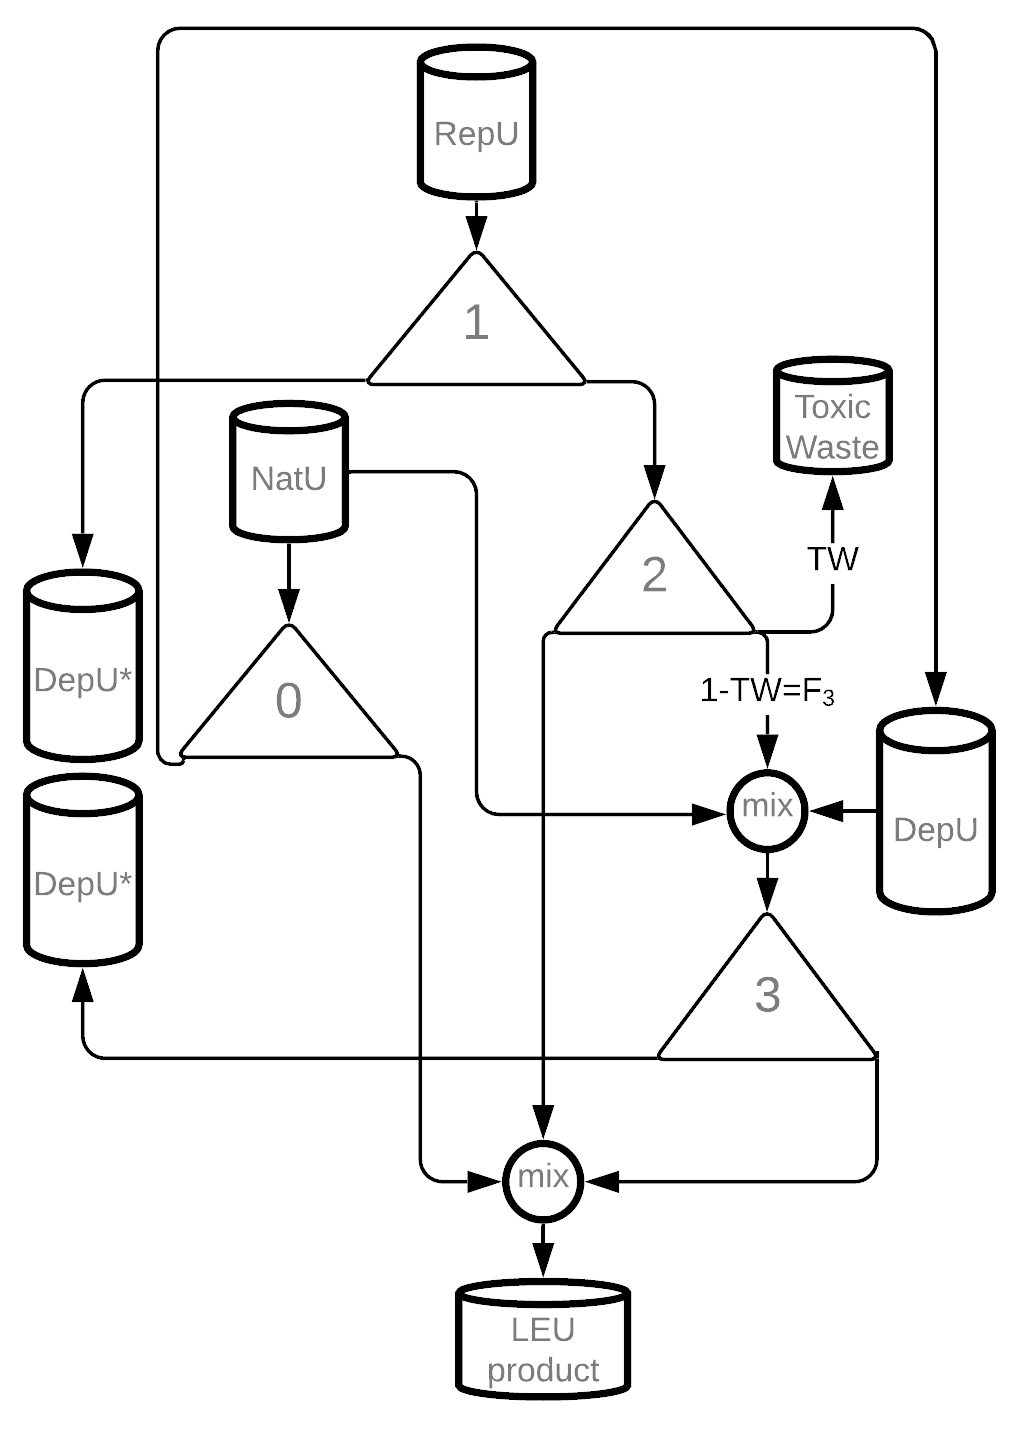
\includegraphics[scale=0.3]{cascades/triple_cascade_complete_return}}
%   \caption{Тройной каскад с подмешиванием НОУ, ОГФУ и природного урана}\label{fig:patent}
% \end{figure}

% Как мы видим, такие схемы также очень ценны как инструмент для переработки предписанного количества выделенного из ОЯТ урана.

Так как наиболее ценны схемы, которые решают вопрос включения побочной легкой фракции в производство свежего НОУ, в качестве альтернатив могут быть рассмотрены следующие схемы.

Одним из вариантов утилизации побочной легкой фракции, образующейся во втором каскаде схемы рис. \ref{fig:vestnik}, является возможность смешать этот побочный продукт с обедненным ураном и отправить на последующее длительное хранение \cite{vodolazskihSposobIzotopnogoVosstanovleniya}. Здесь поток легкой фракции второго каскада разбавляется обедненным гексафторидом из имеющихся складских запасов (дважды обедненным, с низким содержанием $^{235}$U $\approx$0,1\%), отправляя полученную ядерно-безопасную смесь на длительное хранение. Недостатки этого метода заключаются в том, что, хотя этот подход позволяет полностью решить проблему накопления загрязненных отходов $^{232}$U, он вынуждает использовать значительные объемы обедненного гексафторида (в $\approx$50 раз больше, чем разбавляемая им изотопная смесь), а также как тот факт, что значительная масса целевого изотопа $^{235}$U будет потеряна для возможности применения в производстве свежего НОУ, что снизит эффективность использования переработанного урана, которая выражается в степени извлечения $^{235}$U из регенерата. Степень извлечения этого изотопа для схемы двойного модифицированного каскада может быть записана как
$U^{235}_{Rec} = \frac{P \cdot C_{P}^{235}}{F_0 \cdot C_{NatU}^{235} + E \cdot C_{E}^{235}}$, где массовые потоки $P$, $E$ и $F_0$ умножены на концентрации $^{235}$U в этих потоках.

Тогда как в таком варианте предлагается избавиться от радиоактивного материала с высокой концентрацией $^{232}$U путем разбавления его обедненным гексафторидом и последующей отправкой на хранение, помимо методов, позволяющих избежать его накопления, применяя его для конечного производства НОУ, таких как тройные схемы \cite{smirnovMethodEnrichReprocessed2019}, существует вариант направить поток легкой фракции на питание другого двойного каскада, производящего НОУ для последующего цикла \cite{nevinicaToplivnyyCiklLegkovodnogo2019}. Такую схему  каскада целесообразно использовать в условиях многократного рецикла урана, начиная со второго рецикла, а также в условиях постоянного производства регенерированного топлива для парка реакторов на тепловых нейтронах. Устройство этой схемы, изображенной на рис. \ref{P2utilizationRing} предлагает вовлекать этот материал после его накопления в результате обогащения изначальной партии регенерата $E$, поступившей на обогатительное производство в обогащение следующей партии регенерированного урана $E'$ из переработанных ОТВС. Показано, что реализация предлагаемой схемы позволяет полностью израсходовать как вновь поступивший на повторное обогащение регенерированный уран, так и проблемный промежуточный продукт $P_2$, оставшийся после прошлой операции по дообогащению -- гексафторид высокообогащенного урана с относительно высоким содержанием $^{232}$U.

\begin{figure}[ht]
  \centerfloat{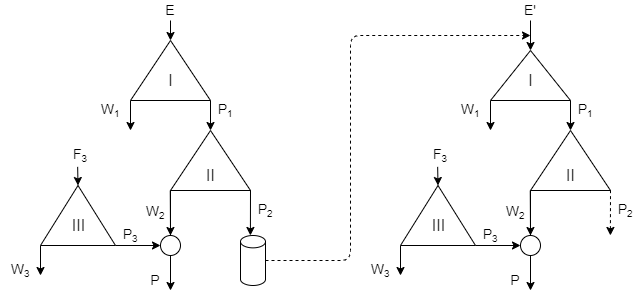
\includegraphics[scale=0.7]{cascades/P2utilizationRing}}
  \caption{Схема передачи загрязненной изотопом $^{232}$U фракции гексафторида урана в двойном каскаде от первой партии дообогащенного регенерированного урана к последующей.}\label{P2utilizationRing}
\end{figure}

Процесс возврата данного материала в воспроизводство низкообогащенного урана может быть начат практически после дообогащения регенерата уже для одной ТВС и даже для ее части (непрерывный возврат), схема каскада при этом преобразуется к виду, когда проблемный промежуточный продукт $P_2$ возвращается и подмешивается к потоку питающего исходного регенерата $E$.

Очевидно, что при использовании предлагаемой схемы и непрерывной работе завода по обогащению, удастся полностью замкнуть топливный цикл по урану, а единственным отходом производства станет только обедненный гексафторид, образующийся в отвале первого каскада. Однако данный продукт можно считать штатным отходом
обогатительного производства, для которого на сегодняшний день отработаны технологии хранения и переработки. При этом после вывода завода из эксплуатации (или остановки на планово-предупредительный ремонт) останется невостребованным только тот объем обогащенного по изотопу $^{232}$U гексафторида урана, который будет образован после обогащения последней партии регенерата на этом заводе. Таким образом, предлагаемый в настоящей статье подход к дообогащению регенерата урана позволяет организовать полный возврат регенерированного урана в топливный цикл в течение практически всего жизненного цикла топлива легководных реакторов,
работающих в замкнутом топливном цикле, как показывают результаты работы \cite{nevinicaToplivnyyCiklLegkovodnogo2019}.

\section{Вариант независимой утилизации побочного продукта легкой фракции второго каскада}

В следующей работе [PNE 2021] предлагается способ обращения с $P_2$, который позволяет использовать полезный потенциал его $^{235}$U в качестве независимого ресурса. Предлагаемая схема направлена на решение следующих задач.

\begin{enumerate}
  \item Сокращение доли потребляемого обедненного урана при сохранении возможности использования высокообогащенного побочного продукта.
  \item Обеспечение полного возврата регенерированного урана в топливный цикл.
  \item Повышение степени вовлечения делящегося изотопа$^{235}$U из регенерата.
  \item Минимизация расхода природного урана на производство единицы свежего топлива для загрузки легководного реактора.
\end{enumerate}

Вариант, который рекомендуется статье [PNE 2021], касается уже накопленных побочных продуктов двойного каскада. Здесь на рис. \ref{P2utilization}, легкая фракция $P_2$  разбавляется обедненным  $F_{du}$ (du -- depleted uranium -- обедненный уран) до уровня $^{235}$U, необходимого в продукте, с добавкой, которая учитывает компенсацию $^{236}$U. Полученную смесь разбавляют низкообогащенным ураном  $F_{leu}$ (leu -- низкообогащенный уран) , полученным из природного урана, в пропорции для достижения соответствия содержания $^{232}$U в конечном продукте $F_{add}$ пороговому значению.

\begin{figure}[ht]
  \centerfloat{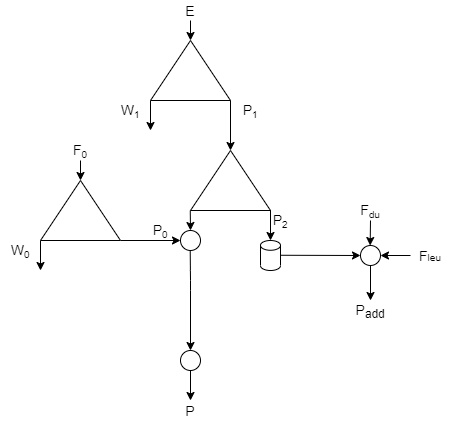
\includegraphics[scale=0.7]{cascades/P2utilization}}
  \caption{Схема независимого вовлечения загрязненногой изотопом $^{232}$U фракции с разбавлением обедненным и природным ураном}\label{P2utilization}
\end{figure}

\begin{table}[h]
  \centering
  \normalsize\begin{tabulary}{1.0\textwidth}{CCCCC}
  $^{232}$U & Цикл № & $P_2$, кг & Дополнительный продукт из $P_2$, доля новой ТВС, \% & Экономия природного урана, \% \\
  1.e-6\% & 2 & 1.09 & 7.11 & 14.6 \\
   & 5 & 0.92 & 10.21 & 6.3 \\
  5.e-7\% & 2 & 1.33 & 14.22 & 7.3 \\
   & 5 & 0.92 & 20.42 & 3.1 \\
  \end{tabulary}
  \caption{{Результаты вовлечения $P_2$ в производство дополнительного НОУ-продукта{\label{independent}}%
  }}
\end{table}

Принимая во внимание, что в конечном продукте двойного каскада НОУ-продукт требуемого качества был произведен в количестве, необходимом для одной ТВС (469 кг), масса $P_2$ и вклад этого побочного продукта в производство дополнительной ТВС приведены в табл. \ref{independent}. Так, значения в столбце <<Дополнительный продукт из $P_2$, доля новой ТВС \%>> соответствуют доле дополнительно произведенного НОУ из побочного $P_2$, образовавшегося в процессе обогащения топлива из регенерата для одной ТВС (469 кг).
Как мы могли видеть, предлагаемый способ использования $P_2$ позволяет экономить большее количество природного урана, чем двойной модифицированный каскад, в котором не предполагается задействование этого материала. Такой эффект более значителен для случаев, когда приходится иметь дело с побочным продуктом двойного каскада, образующимся на начальных циклах повторного использования (второй цикл в табл. \ref{independent}). Такая схема также показывает себя как более предпочтительная в экономии природного урана (вдвое выигрышнее, согласно табл. \ref{independent}), когда ПДК $^{232}$U получаемого таким способом продукта задается на уровне в два раза выше ($1\cdot10^{-7}$\% вместо $5\cdot10^{-7}$\%). Важно также показать следующие соотношения. Тогда как накопленный побочный продукт $P_2$ можно было бы использовать для производства дополнительных $\approx$7\% свежего НОУ-продукта для новой топливной сборки, это соответсвует возможности произвести дополнительную 15-ю сборку из накопленного $P_2$, образовавшегося при производстве предыдущих четырнадцати ТВС. Таким образом, для современного легководного реактора, такого как, например, российский ВВЭР-1200 или европейский PWR, где активная зона состоит из более чем 150 тепловыделяющих сборок, было бы изготовить дополнительно более 10 ТВС, взяв за основу предложенный способ. Значение экономии природного урана здесь соответствует доле $P_2$, смешанной с обедненным ураном $F_{du}$, до того, как он будет смешан с НОУ-разбавителем $F_{leu}$, полученным из природного урана. Эта пропорция также соответствует экономии на работы разделения, которая была бы затрачена в случае использования прямого обогащения природного урана в ординарном каскада без привлечения $P_2$.

Следует отметить, что рассмотренная схема имеет преимущество перед тройным каскадом (рис. \ref{fig:Tomsk}), заключающееся в том, что радиоактивными изотопами $^{232}$U и $^{234}$U будет загрязнена меньшая доля разделительного оборудования, поскольку в случае независимого вовлечения $P_2$, предложенного в диссертации, им не загрязняется дополнительные сепарационные мощности (газовые центрифуги).

\clearpage